\documentclass[utf8]{article}

%\usepackage{doi}
\usepackage{authblk}
\usepackage[T1]{fontenc}
\usepackage[utf8]{inputenc}
\usepackage[pdftex]{xcolor}
\usepackage[pdftex]{graphicx}
\usepackage[authoryear,round]{natbib}

% review mode
\usepackage{geometry}
\usepackage{lineno}
\linenumbers
\linespread{1.5}

% custom colours
\definecolor{darkblue}{cmyk}{0.9,0.3,0.0,0.0}
\definecolor{darkgreen}{cmyk}{0.8,0.0,1.0,0.0}
\definecolor{darkred}{cmyk}{0.1,0.9,0.8,0.0}
\definecolor{darkorange}{cmyk}{0.0,0.5,1.0,0.0}
\definecolor{darkpurple}{cmyk}{0.6,0.7,0.0,0.0}
\definecolor{darkbrown}{cmyk}{0.23,0.73,0.98,0.12}

% custom commands
\newcommand{\idea}[1]{\textcolor{darkgreen}{\emph{[\textbf{IDEA:} #1]}}}
\newcommand{\note}[1]{\textcolor{darkblue}{\emph{[\textbf{NOTE:} #1]}}}
\newcommand{\todo}[1]{\textcolor{darkred}{\emph{[\textbf{TODO:} #1]}}}
\newcommand{\aref}[0]{\textcolor{darkblue}{\textbf{[REF.]}}}

\graphicspath{{../../figures/}}

\title{Last glacial cycle glacier erosion potential in the Alps}
\author{Julien Seguinot}
\affil{Anafi, Greece}


% ======================================================================
\begin{document}
% ======================================================================

\maketitle

\begin{abstract}

    The glacial landscape of the Alps has fascinated generations of explorers,
    artists, mountaineers and scientists with its diversity, including
    erosional features of all scales from high-mountain cirques, to steep
    glacial valleys and large overdeepenings. Using previous glacier modelling
    results, and modern observations of bedrock erosion under glaciers, we
    infer a distribution of potential glacier erosion in the Alps over the last
    glacial cycle from 120\,000 years ago to the present.
    %
    Depsite large uncertainties related to the climate history of the Alps and
    glacier erosion processes, the resulting modelled patterns of glacier
    erosion shows persistent features (hopefully). The cumulative imprint of
    the last glacial cycle shows peak erosion at the mouth of the large Alpine
    valleys where glaciers are modelled to have flown with the highest
    velocity. The modelled erosion pattern varies significantly through the
    glacial cycle, but surprisingly the total rate of glacier erosion is
    modelled to be relatively stable during the entire glacial cycle.  While
    glacial maxima lead to high erosion rates at low elevations, the
    high-elevation areas are typically preserved under cold-based ice during
    these periods, but are modelled to have experience mode intense erosion
    during periods of intermediate glaciation extent.
    %
    This result indicate that different landscapes of the same mountain range
    most likely correspond to different tmie periods, and explains the
    diversity of glacial landscapes in the Alps.

\end{abstract}

% ----------------------------------------------------------------------
\section{Introduction}
% ----------------------------------------------------------------------

    The glacial landscape of the Alps has fascinated generations of explorers,
    artists, mountaineers and scientists for centuries.

    In fact, the global obsession for the Alps has been so large that in
    English, a non-native language foreign to the Alps, the word “alpine” is
    now used to describe any glacially modified mountain landscape worldwide.

    Understanding the beauty of Alpine glacial landscape through the rigour of
    scientific research is yet another endeavour.

    While it has long been understood that glaciers leave a specific imprint on
    the landscape they lie on, observing and quantifying the long-term erosion
    and sedimentation processes has been a challenge. While some regions are
    specifically characterised by cirque glaciation (), or glacial scouring (),
    the European Alps present a variety of glacial landforms with a density
    seen in few other places on Earth.

    It is typically assumed that the degree of glacial modification is a proxy
    for the duration of past glacier cover. However glacier sliding velocities
    vary by several orders of magnitude, and erosion laws can be non-linear.
    Besides, cold-based glaciers have been shown to preserve landscape.

    Fig.~\ref{fig:landscape} -- Alpine glacial erosion landscape photos.

% ----------------------------------------------------------------------
\section{Methods}
% ----------------------------------------------------------------------

% -- -- -- -- -- -- -- -- -- -- -- -- -- -- -- -- -- -- -- -- -- -- -- -
\subsection{Ice sheet modelling}
% -- -- -- -- -- -- -- -- -- -- -- -- -- -- -- -- -- -- -- -- -- -- -- -

% -- -- -- -- -- -- -- -- -- -- -- -- -- -- -- -- -- -- -- -- -- -- -- -
\subsection{Erosion law}
% -- -- -- -- -- -- -- -- -- -- -- -- -- -- -- -- -- -- -- -- -- -- -- -

% ----------------------------------------------------------------------
\section{Results}
% ----------------------------------------------------------------------

% -- -- -- -- -- -- -- -- -- -- -- -- -- -- -- -- -- -- -- -- -- -- -- -
\subsection{Cumulative erosion}
% -- -- -- -- -- -- -- -- -- -- -- -- -- -- -- -- -- -- -- -- -- -- -- -

    Fig.~\ref{fig:cumulative} -- Cumulative erosion.

% -- -- -- -- -- -- -- -- -- -- -- -- -- -- -- -- -- -- -- -- -- -- -- -
\subsection{Temporal evolution}
% -- -- -- -- -- -- -- -- -- -- -- -- -- -- -- -- -- -- -- -- -- -- -- -

    Fig.~\ref{fig:transects} -- Erosion rate along transects.

    Fig.~\ref{fig:evolution} -- Erosion rate and ice volume.

    Fig.~\ref{fig:hypsogram} -- Erosion rate and elevation.

% ----------------------------------------------------------------------
\section{Discussion}
% ----------------------------------------------------------------------

% -- -- -- -- -- -- -- -- -- -- -- -- -- -- -- -- -- -- -- -- -- -- -- -
\subsection{Erosion uncertainties}
% -- -- -- -- -- -- -- -- -- -- -- -- -- -- -- -- -- -- -- -- -- -- -- -

    Fig.~\ref{fig:uncertainty} -- Erosion uncertainties

% -- -- -- -- -- -- -- -- -- -- -- -- -- -- -- -- -- -- -- -- -- -- -- -
\subsection{Sensitivity to climate}
% -- -- -- -- -- -- -- -- -- -- -- -- -- -- -- -- -- -- -- -- -- -- -- -

    Fig.~\ref{fig:sensitivity} -- Sensitivity to climate.

% ----------------------------------------------------------------------
\section{Conclusions}
% ----------------------------------------------------------------------

% ----------------------------------------------------------------------
% Acknowledgements
% ----------------------------------------------------------------------

%\paragraph{Acknowledgements}
%\paragraph{Author contributions}
%\paragraph{Conflict of interest}
%\paragraph{Contribution to the field}
%\paragraph{Data availability}


% ----------------------------------------------------------------------
% References
% ----------------------------------------------------------------------

\bibliographystyle{abbrvnat}
\bibliography{../../../references/references}


% ----------------------------------------------------------------------
% Figures
\clearpage
% ----------------------------------------------------------------------

    \begin{figure*}
      \centerline{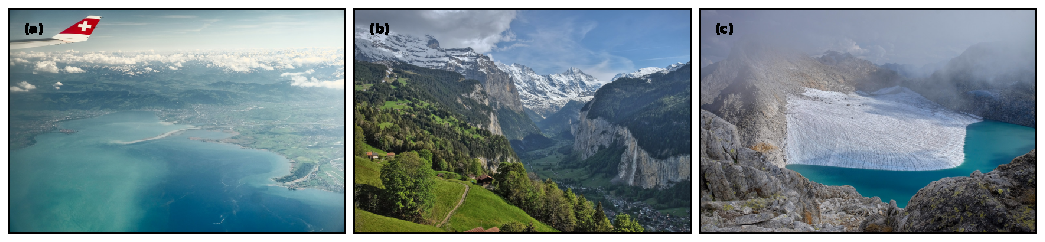
\includegraphics{alpero_landscape}}
      \caption{%
        Alpine glacial erosion landscape diversity.
        \textbf{(a)} Piedmont overdeepening of Lake Constance, ca.~10x50\,km.
        \textbf{(b)} Glacial trough of Lauterbrunnental, ca.~1x10\,km.
        \textbf{(c)} Mountain cirque of Chüebodengletscher, ca.~1x1\,km.}
      \label{fig:landscape}
    \end{figure*}

    \begin{figure*}
      \centerline{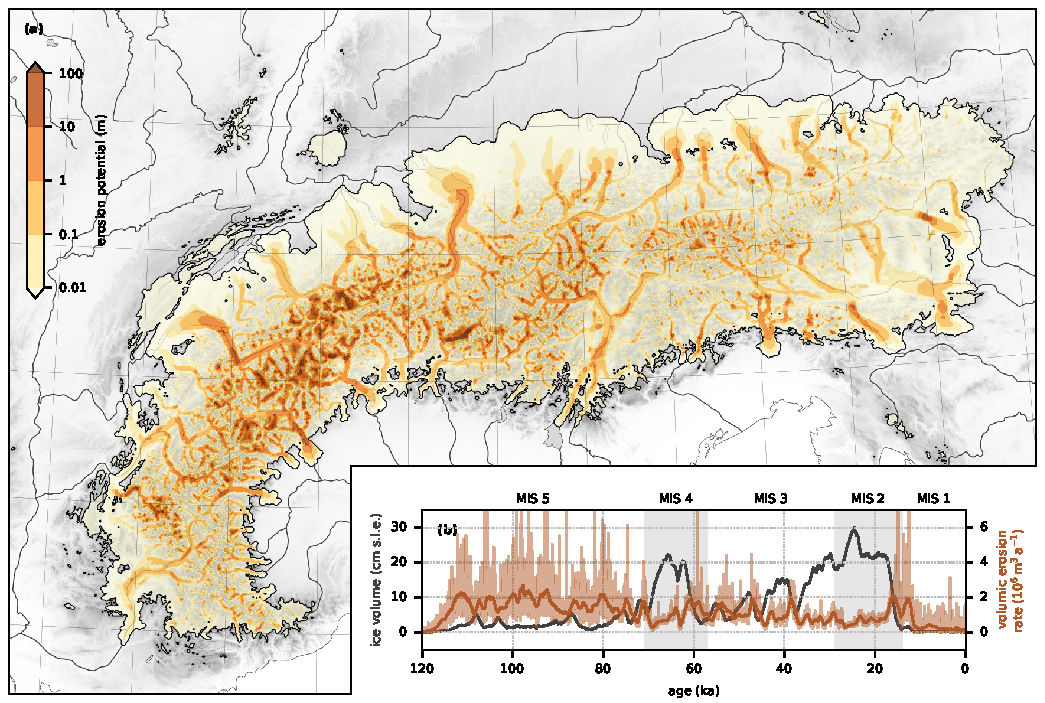
\includegraphics{alpero_cumulative}}
      \caption{%
        \textbf{(a)} Modelled cumulative (time-integrated) glacial erosion
          potential over the last glacial cycle.
        \textbf{(b)} Modelled total ice volume in centimetres of sea-level
          equivalent (cm~s.l.e., black), volumic (domain-integrated) erosion
          rate (light brown) and 100-a running mean (dark brown). Shaded gray
          areas indicate the timing for MIS~2 and~4
          \citep{Lisiecki.Raymo.2005}.} \label{fig:cumulative}
    \end{figure*}

    \begin{figure}
      \centerline{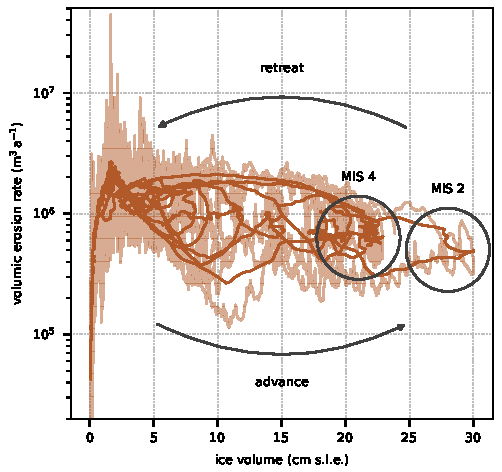
\includegraphics{alpero_evolution}}
      \caption{%
        Modelled volumic (domain-integrated) erosion rate (light brown) and 100-a
        running mean (dark brown) in relation to modelled total ice volume in
        centimetres of sea-level equivalent (black).}
      \label{fig:evolution}
    \end{figure}

    \begin{figure*}
      \centerline{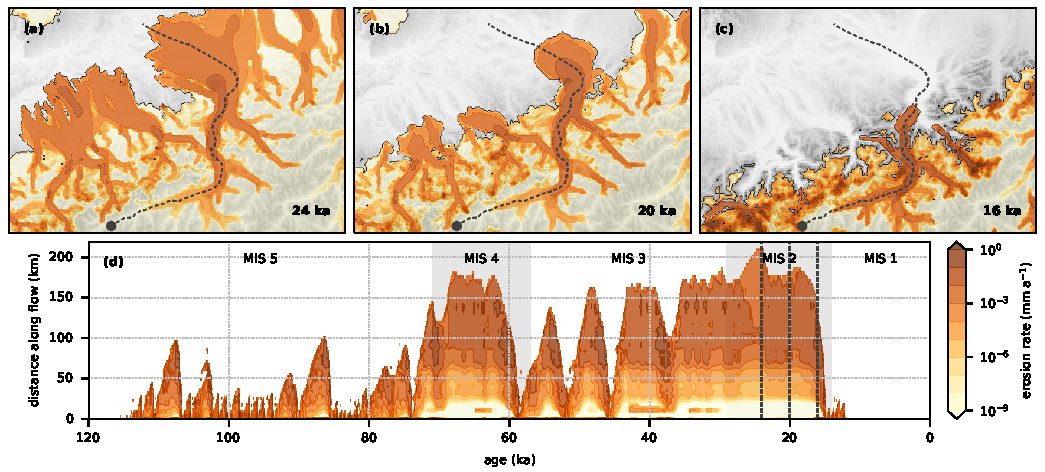
\includegraphics{alpero_transects}}
      \caption{%
        \textbf{(a, b, c)} Modelled instantaneous erosion rate of the Rhine
          Glacier for selected post-Last Glacial Maximum ages.
        \textbf{(d)} Interpolated instantaneous erosion rate along a Rhine
          Glacier transect for the entire last glacial cycle (upper panels
          dashed line).}
      \label{fig:transects}
    \end{figure*}

    \begin{figure*}
      \centerline{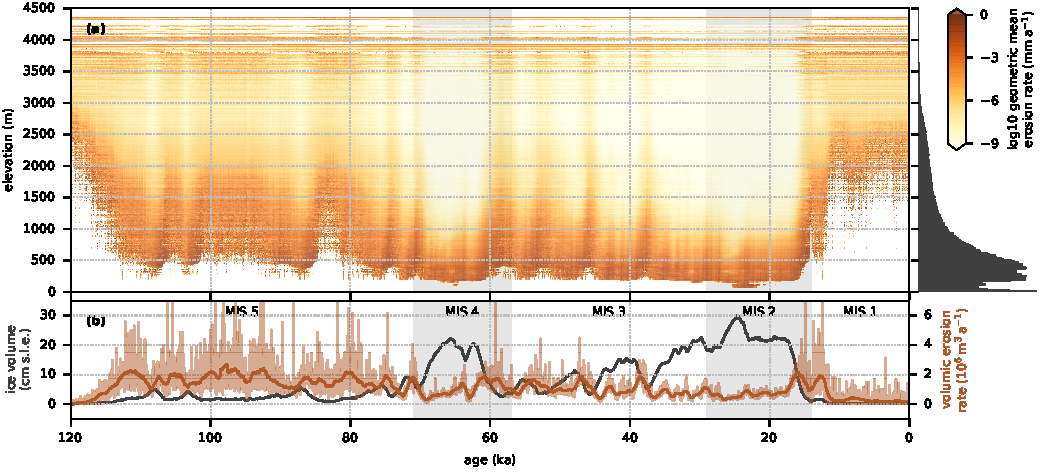
\includegraphics{alpero_hypsogram}}
      \caption{%
        \textbf{(a)} Modelled erosion rate ``hypsogram'', showing the geometric
          mean of (non-zero) modelled erosion rates in 10-m elevation bands
          across the entire model domain and its time evolution.
        \textbf{(b)} Same as Fig.~\ref{fig:cumulative}b.}
      \label{fig:hypsogram}
    \end{figure*}

    \begin{figure*}
      \centerline{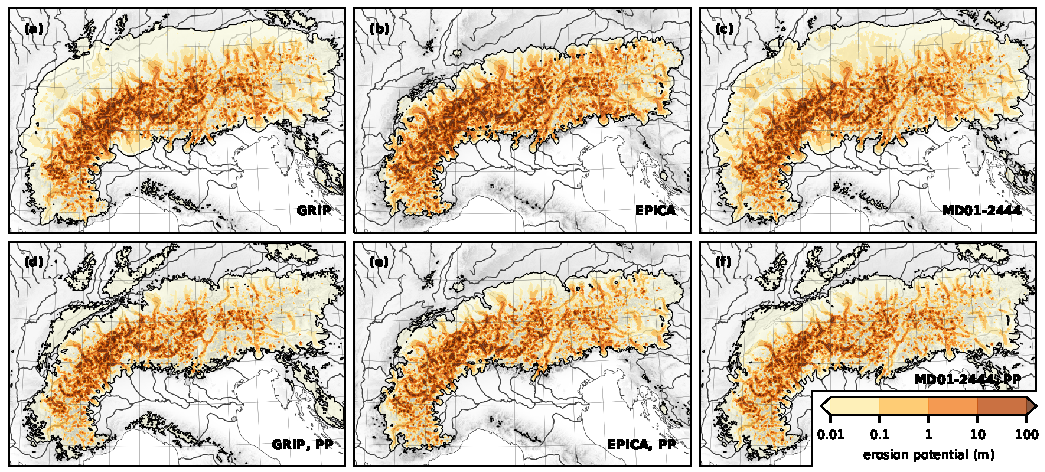
\includegraphics{alpero_sensitivity}}
      \caption{%
        Modelled cumulative glacial erosion potential over the last glacial
        cycle without \textbf{(a, b, c)} and with \textbf{(d, e, f)}
        paleo-precipitation corrections, and using three different
        palaeo-temperature histories \citep[see][]{Seguinot.etal.2018}.}
      \label{fig:sensitivity}
    \end{figure*}

    \begin{figure*}
      \centerline{\includegraphics{alpero_uncertainty}}
      \caption{%
        Modelled cumulative (time-integrated) glacial erosion potential for
        three different erosion laws published by
        \textbf{(a)} \citet{Cook.etal.2020},
          $1.665 \times 10^{-1} \textbf{u}_\mathrm{b} ^{0.6459}$,
        \textbf{(b)} \citet{Herman.etal.2015},
          $2.7 \times 10^{-7} \textbf{u}_\mathrm{b} ^{2.02}$
          (same as Fig.~\ref{fig:cumulative}a), amd
        \textbf{(c)} \citet{Koppes.etal.2015},
          $5.2 \times 10^{-8} \textbf{u}_\mathrm{b} ^{2.34}$.
        \textbf{(d)} Corresponding erosion power laws, and
        \textbf{(e)} modelled cumulative (time-integrated) glacial erosion
          potential along a Rhine Glacier transect (upper panels dashed line).}
      \label{fig:uncertainty}
    \end{figure*}

% ----------------------------------------------------------------------
% Tables
%\clearpage
% ----------------------------------------------------------------------


% ======================================================================
\end{document}
% ======================================================================
